\pdfminorversion=4
\documentclass{beamer}
%%%%%%%%%%%%%%%%%%%%%%%%%%%%%%%%%%%%%%%%%%%%%%%%%%%%%%%%%%%%%%%%%%%%%%%%%%%%%%%%%%%%%%%%%%%%%%%%%%%%%%%%%%%%%%%%%%%%%%%%%%%%%%%%%%%%%%%%%%%%%%%%%%%%%%%%%%%%%%%%%%%%%%%%%%%%%%%%%%%%%%%%%%%%%%%%%%%%%%%%%%%%%%%%%%%%%%%%%%%%%%%%%%%%%%%%%%%%%%%%%%%%%%%%%%%%
\usepackage{amssymb}
\usepackage{mathpazo}
\usepackage{multimedia}
\usepackage{amsfonts}
\usepackage{amsmath}
\usepackage{hyperref}
\usepackage{listings}

\setcounter{MaxMatrixCols}{10}

\hypersetup{
colorlinks = true,
allcolors = blue,
}
\definecolor{mygreen}{rgb}{0,0.6,0}
\newtheorem{prop}{Proposition}
\newcommand{\E}{\mathbb{E}}
\newcommand{\I}{\mathbb{I}}
\setbeamertemplate{footline}[frame number]
\setbeamertemplate{navigation symbols}{}
\setbeamertemplate{mini frames}{}
\setbeamertemplate{itemize item}[ball]
\setbeamertemplate{itemize subitem}[ball]
\setbeamercovered{invisible}
\renewcommand{\baselinestretch}{1.2}
\small\normalsize
\subtitle{A simple two-period model}
\institute[Universities Here and There]{University of Birmingham}
%\input{tcilatex}

%%%%%%%%%%%%%%%%%%%%%%%%%%%%%%%%%%%%%%%%%%%%%%%%%%%%%%%%
\begin{document}

\title{Advanced Numerical Methods}
\subtitle{Solving DSGE Models with Dynare, Part 2}
\author{Alessandro~Di Nola}
\date{}

\begin{frame}
\titlepage
\end{frame}

%\section{Notation}

%TCIMACRO{\TeXButton{BeginFrame}{\begin{frame}}}%
%BeginExpansion
\begin{frame}%
%EndExpansion
\frametitle{Outline}

\begin{itemize}
\item How to install and run Dynare

\item Introduction to Dynare

\item Incorporating Dynare in other Matlab programs

\item Peculiarities of Dynare and advanced tricks

\item Impulse Response Functions

\item Stochastic simulations

%\item Perturbation and the effect of uncertainty on the solution

%\item Higher order perturbation

\end{itemize}

%TCIMACRO{\TeXButton{EndFrame}{\end{frame}}}%
%BeginExpansion
\end{frame}%
%EndExpansion

%TCIMACRO{\TeXButton{BeginFrame}{\begin{frame}}}%
%BeginExpansion
\begin{frame}%
%EndExpansion
\frametitle{References}

\begin{itemize}

\item Of course, Dynare's reference manual:

\begin{itemize}
	\item Adjemian, S. et al., 2011. ``\textcolor{blue}{Dynare: Reference Manual Version 7},'' Dynare Working Papers 1, CEPREMAP, revised Jul 2018.
\end{itemize}

\item A good textbook treatment is provided in: Miao, J., 2014 ``Economic Dynamics in Discrete Time,'' MIT Press. Especially chapters 2.5 and 15.

\item Lots of material on the web about Dynare

\begin{itemize}
	\item \texttt{https://forum.dynare.org/}
\end{itemize}

\end{itemize}

\end{frame}
%%%%%%%%%%%%%%%%%%%%%%%%%%%%%%%%%%%%%%%%%%%%%%%%%%%%%%%%

\begin{frame}[fragile]
\frametitle{How to install and run Dynare}

\textbf{To install it:}
\begin{itemize}
	\item Go to the Dynare website: \texttt{https://www.dynare.org/}.
	\item In the main menu, go to ``Download''.
	\item Download current stable release
	\begin{itemize}
		\item Available for Windows, Mac, Linux.
	\end{itemize}
    \item Run the executable. It will install Dynare in your C drive.
    \item Start Matlab, click in the file menu on ``set path''.
    \item Click on the button ``Add folder''. \textcolor{red}{Warning}: DO NOT select ``Add with Subfolders''.
    \item Select the matlab subdirectory of your Dynare installation. For ex., select: 
    \begin{verbatim}
    C:\dynare\4.5.7\matlab
    \end{verbatim}
    \item Apply the setting by clicking ``Save'' button.
\end{itemize}
\end{frame}
%%%%%%%%%%%%%%%%%%%%%%%%%%%%%%%%%%%%%%%%%%%%%%%%%%%%%%%%

\begin{frame}[fragile]
\frametitle{How to install and run Dynare}

\textbf{How to run it:} 
\begin{itemize}
	\item In the Matlab main window, change the directory to the one where you have stored your Dynare model file.
	\item To run the program \texttt{myfile.mod}, type the command:
	\begin{verbatim}
	dynare myfile.mod
	\end{verbatim}	
	\item You can type the above command either in the Matlab command window or in a Matlab script.
	\item \textcolor{red}{Warning}: Dynare clears all variables out of memory. To overrule this, add option ``noclearall'':
	\begin{verbatim}
	dynare myfile.mod noclearall
	\end{verbatim}
\end{itemize}
\end{frame}
%%%%%%%%%%%%%%%%%%%%%%%%%%%%%%%%%%%%%%%%%%%%%%%%%%%%%%%%

\begin{frame}
\frametitle{Stochastic growth model}

\begin{itemize}
	\item Baseline stochastic growth model: Social planner maximizes
	\begin{equation*}
	\mathbb{E}_{0} \sum_{t=0}^{\infty} \beta^{t} \frac{c_{t}^{1-\sigma}}{1-\sigma}
	\end{equation*}
	subject to resource constraint
	\begin{equation*}
	c_{t}+k_{t+1}=z_{t} k_{t}^{\alpha}+(1-\delta) k_{t}
    \end{equation*}
	given productivity
	\begin{equation*}
	\log z_{t+1}=\rho \log z_{t}+\varepsilon_{t+1}, \quad \varepsilon_{t+1} \sim \operatorname{IID} N\left(0, \sigma_{\varepsilon}^{2}\right)
	\end{equation*}
	for some given parameters $ \alpha,\beta,\delta,\rho,\sigma,\sigma_{\varepsilon} $ (here $ \bar{z} = 1 $).
\end{itemize}

\end{frame}
%%%%%%%%%%%%%%%%%%%%%%%%%%%%%%%%%%%%%%%%%%%%%%%%%%%%%%%%

\begin{frame}
\frametitle{Stochastic growth model, cont'd}

\begin{itemize}
\item Planner takes as given beginning-of-period capital $k_{t}$ and current productivity $z_{t}$
\item We say that 
\begin{itemize}
	\item $\left( k_{t},\ z_{t}\right) $ are \textit{endogenous state} variables
\end{itemize}

\item Given $k_{t}$ and $z_{t}$, planner chooses current consumption (and next-period capital $k_{t+1}$ is implied by the resource constraint)
\item We say that
\begin{itemize}
	\item $c_{t}$ is an \textit{endogenous control} variable
\end{itemize}
\end{itemize}

\end{frame}
%%%%%%%%%%%%%%%%%%%%%%%%%%%%%%%%%%%%%%%%%%%%%%%%%%%%%%%%

\begin{frame}
\frametitle{Stochastic growth model, cont'd}

\begin{itemize}
\item Let's do some book-keeping

\item In total, we have \textit{three} \textit{endogenous variables}:%
\begin{equation*}
\left\{ c_{t},k_{t},z_{t}\right\} 
\end{equation*}

\item We need \textit{three model equations}:%
\begin{equation*}
c_{t}+k_{t+1}=z_{t}k_{t}^{\alpha }+(1-\delta )k_{t}\text{ (Resource
constraint)}
\end{equation*}%
\begin{equation*}
\log z_{t+1}=\rho \log z_{t}+\varepsilon _{t+1}\text{ (AR1 productivity)}
\end{equation*}%
\begin{equation*}
c_{t}^{-\sigma }=\beta \mathbb{E}_{t}\left\{ c_{t+1}^{-\sigma }\left[
z_{t+1}\alpha k_{t+1}^{\alpha -1}+1-\delta \right] \right\} \text{ (Euler
equation)}
\end{equation*}

\item There is also $\varepsilon _{t}$ which is exogenous
\end{itemize}
\end{frame}
%%%%%%%%%%%%%%%%%%%%%%%%%%%%%%%%%%%%%%%%%%%%%%%%%%%%%%%%

\begin{frame}
\frametitle{Dynare model file}

The structure of a Dynare model file (\texttt{.mod})
\begin{enumerate}
	\item Declare endogenous variables
	\item Declare exogenous variables
	\item Declare parameters
	\item Declare the model equations
	\item Ask Dynare to solve for the steady state
	\item Ask Dynare to solve for the the dynamics
\end{enumerate}
\end{frame}
%%%%%%%%%%%%%%%%%%%%%%%%%%%%%%%%%%%%%%%%%%%%%%%%%%%%%%%%

\begin{frame}[fragile]
\frametitle{(1) Declare endogenous variables}
%\framesubtitle{subtitle}
\begin{itemize}
	\item From \texttt{stochastic\_growth\_dynare.mod}
	
	\begin{verbatim}
	% (1) declare endogenous variables
	var c, k, z;
	\end{verbatim}
	\item Note productivity $ z_{t} $ is treated as endogenous.
\end{itemize}

\end{frame}
%%%%%%%%%%%%%%%%%%%%%%%%%%%%%%%%%%%%%%%%%%%%%%%%%%%%%%%%

\begin{frame}[fragile]
\frametitle{(2) Declare exogenous variables}
%\framesubtitle{subtitle}
\begin{itemize}
	\item It is the innovations $ \varepsilon $ that are fundamentally exogenous
	
	\begin{verbatim}
		% (2) declare exogenous variables (shocks)
		varexo e;
	\end{verbatim}
	
\end{itemize}
\end{frame}
%%%%%%%%%%%%%%%%%%%%%%%%%%%%%%%%%%%%%%%%%%%%%%%%%%%%%%%%

\begin{frame}[fragile]
\frametitle{(3) Declare parameters}
%\framesubtitle{subtitle}
\begin{itemize}
	\item List of parameter names
	
	\begin{verbatim}
		% (3) declare parameters
		parameters alpha, beta, delta, sigma, rho, sigmaeps;
	\end{verbatim}
	
	\item Set parameter values
	
	\begin{verbatim}
		alpha    = 0.35;
		beta     = 0.95;
		delta    = 0.1;
		rho      = 0.95;
		sigma    = 3.00;
		sigmaeps = 0.01;
	\end{verbatim}
	
	
\end{itemize}
\end{frame}
%%%%%%%%%%%%%%%%%%%%%%%%%%%%%%%%%%%%%%%%%%%%%%%%%%%%%%%%


\begin{frame}[fragile]
\frametitle{Dynare notation for model equations}
\framesubtitle{Resource constraint}
\begin{itemize}
	\item In usual notation
	$$
	c_{t}+k_{t+1}=z_{t} k_{t}^{\alpha}+(1-\delta) k_{t}
	$$
	
	\item In Dynare notation, \textit{supposing we want an approximation in logs}
	\begin{verbatim}
		exp(c) + exp(k)
		= exp(z)*(exp(k(-1))^alpha)+(1-delta)*exp(k(-1));
	\end{verbatim}
	(otherwise approximation will be in levels)
	\item Dynare timing convention:
	\begin{itemize}
		\item Variables chosen at $ t $ have no time argument
		\item Variables chosen at $ t-1 $ have -1 argument
		\item Variables chosen at $ t+1 $ have +1 argument
	\end{itemize}
	
	
\end{itemize}
\end{frame}
%%%%%%%%%%%%%%%%%%%%%%%%%%%%%%%%%%%%%%%%%%%%%%%%%%%%%%%%

\begin{frame}[fragile]
\frametitle{Dynare notation for model equations}
\framesubtitle{Consumption Euler equation}
\begin{itemize}
	\item In usual notation:
	$$
	c_{t}^{-\sigma}=\beta \mathbb{E}_{t}\left\{c_{t+1}^{-\sigma}\left[z_{t+1} \alpha k_{t+1}^{\alpha-1}+1-\delta\right]\right\}
	$$
	\item In Dynare notation, supposing we want an approximation in logs
	
	\begin{verbatim}
	exp(c)^(-sigma)
	= beta*(exp(c(+1))^(-sigma))
	*(alpha*exp(z(+1))*(exp(k)^(alpha-1))+1-delta);
	\end{verbatim}
	
\end{itemize}
\end{frame}
%%%%%%%%%%%%%%%%%%%%%%%%%%%%%%%%%%%%%%%%%%%%%%%%%%%%%%%%

\begin{frame}[fragile]
\frametitle{Dynare notation for model equations}
\framesubtitle{AR(1) for productivity shock}
\begin{itemize}
	\item In usual notation
	$$
	\log z_{t+1}=\rho \log z_{t}+\varepsilon_{t+1}
	$$
	\item In Dynare notation, supposing we want an approximation in logs
	
	\begin{verbatim}
	z = rho*z(-1) + e;
	\end{verbatim}
	
\end{itemize}
\end{frame}
%%%%%%%%%%%%%%%%%%%%%%%%%%%%%%%%%%%%%%%%%%%%%%%%%%%%%%%%

\begin{frame}[fragile]
\frametitle{(4) Declare the model equations}
%\framesubtitle{subtitle}
\begin{itemize}
	\item Start block with \textbf{model}, then list equations, then \textbf{end}
	
	\begin{verbatim}
	model;
	% resource constraint
	exp(c) + exp(k)
	= exp(z)*(exp(k(-1))^alpha)+(1-delta)*exp(k(-1));
	% consumption Euler equation
	exp(c)^(-sigma)
	= beta*(exp(c(+1))^(-sigma))
	*(alpha*exp(z(+1))*(exp(k)^(alpha-1))+1-delta);
	% law of motion productivity
	z = rho*z(-1) + e;
	end;
	\end{verbatim}
	
	
\end{itemize}
\end{frame}
%%%%%%%%%%%%%%%%%%%%%%%%%%%%%%%%%%%%%%%%%%%%%%%%%%%%%%%%

\begin{frame}[fragile]
\frametitle{(5) Solve for the steady state}
%\framesubtitle{subtitle}
\begin{itemize}
	\item Solve for steady state numerically (system of nonlinear equations)
	\item Start block with \textbf{initval}, then list guess, then \textbf{end}
	\begin{verbatim}
	% (5) solve the steady state
	initval;
	c = 0.75;
	k = 3;
	z = 1;
	e = 0;
	end;
	steady;
	\end{verbatim}
	\item Can enter exact solution here if you have one
	\item Given model equations that we declared, steady-state is in \textit{logs}.
\end{itemize}
\end{frame}
%%%%%%%%%%%%%%%%%%%%%%%%%%%%%%%%%%%%%%%%%%%%%%%%%%%%%%%%

\begin{frame}[fragile]
\frametitle{Set the shocks}
%\framesubtitle{subtitle}
\begin{itemize}
	\item Set the variance/covariance structure of shocks
	\begin{verbatim}
	% specify variance of shocks
	shocks;
	var e = 100*sigmaeps^2;
	end;
	\end{verbatim}
	\item Only one shock here so this is simple.
	\item Later: example with two correlated shocks.
\end{itemize}
\end{frame}
%%%%%%%%%%%%%%%%%%%%%%%%%%%%%%%%%%%%%%%%%%%%%%%%%%%%%%%%

\begin{frame}[fragile]
\frametitle{(6) Solve for the dynamics}
%\framesubtitle{subtitle}
\begin{itemize}
	\item Solve for coefficients, obtain moments, plot impulse responses, etc.
	\begin{verbatim}
	% (6) solve the dynamics
	stoch_simul(order=1,irf=100);
	\end{verbatim}
	\item Lots of options available (see user guide for details).
	\item Order of the Taylor approximation: \texttt{order = 1,2,3}.
	\item \textcolor{red}{Note}: the default is \texttt{order = 2}.
\end{itemize}
\end{frame}
%%%%%%%%%%%%%%%%%%%%%%%%%%%%%%%%%%%%%%%%%%%%%%%%%%%%%%%%

\begin{frame}[fragile]
\frametitle{(6) Solve for the dynamics}
\framesubtitle{Impulse responses and simulations}
\begin{itemize}
	\item Setting \texttt{irf = 0} suppresses the plotting of IRFs (useful if you nest Dynare into another Matlab program):
	
	\begin{verbatim}
	stoch_simul(order=1,IRF=0)
	\end{verbatim}
	
	\item Don't plot IRFs, don't print the correlation matrix, don't print moments of the endo variables:
	
	\begin{verbatim}
	stoch_simul(order=1,nocorr,nomoments,irf=0);
	\end{verbatim}
	
	\item Don't print the graphs. Useful for loops.
	
	\begin{verbatim}
	stoch_simul(order=1,nograph,irf=100);
	\end{verbatim}
	
	\item Don't print anything. Useful for loops.
	
	\begin{verbatim}
	stoch_simul(order=1,noprint,irf=100);
	\end{verbatim}
	
\end{itemize}
\end{frame}
%%%%%%%%%%%%%%%%%%%%%%%%%%%%%%%%%%%%%%%%%%%%%%

\begin{frame}[fragile]
\frametitle{Dynare output}
\framesubtitle{Steady-state results}

\begin{verbatim}
STEADY-STATE RESULTS:

c 		 0.186403
k 		 1.27678
z 		 0
\end{verbatim}
\begin{itemize}
	\item Note: Given model equations we have declared, steady state is in logs.
\end{itemize}
\end{frame}
%%%%%%%%%%%%%%%%%%%%%%%%%%%%%%%%%%%%%%%%%%%%%%%%%%%%%%%%

\begin{frame}[fragile]
\frametitle{Dynare output}
\framesubtitle{Policy and transition functions}

\begin{verbatim}
POLICY AND TRANSITION FUNCTIONS
            c               k               z
Constant    0.186403        1.276779               0
k(-1)       0.382458        0.924091               0
z(-1)       0.676055        0.187070        0.950000
e           0.711637        0.196916        1.000000
\end{verbatim}


\begin{itemize}
	\item Policy functions produced by Dynare are slightly different from what we are used to.
	\item Dynare artificially splits $ z_{t} $ into predetermined component and an exogenous component.
	
\end{itemize}
\end{frame}
%%%%%%%%%%%%%%%%%%%%%%%%%%%%%%%%%%%%%%%%%%%%%%%%%%%%%%%%
\begin{frame}[fragile]
\frametitle{Dynare output}
\framesubtitle{Policy and transition functions}

\begin{verbatim}
POLICY AND TRANSITION FUNCTIONS
            c               k               z
Constant    0.186403        1.276779               0
k(-1)       0.382458        0.924091               0
z(-1)       0.676055        0.187070        0.950000
e           0.711637        0.196916        1.000000
\end{verbatim}


\begin{itemize}
	\item What we are used to see:
	$$ \tilde{c}_{t} =\psi_{c k} \tilde{k}_{t-1}+\psi_{c z} \tilde{z}_{t} $$
	\item What Dynare spits out:
	$$ \log c_{t} =\log \overline{c}+\psi_{c k} (\log k_{t-1}-\log \overline{k})+\left(\psi_{c z} \rho\right) \log z_{t-1}+\psi_{c z} \varepsilon_{t}$$
\end{itemize}
\end{frame}
%%%%%%%%%%%%%%%%%%%%%%%%%%%%%%%%%%%%%%%%%%%%%%

\begin{frame}[fragile]
\frametitle{Dynare output}
\framesubtitle{Theoretical moments}

\begin{verbatim}
THEORETICAL MOMENTS
VARIABLE         MEAN  STD. DEV.   VARIANCE
c              0.1864     0.4458     0.1987
k              1.2768     0.6471     0.4187
z              0.0000     0.3203     0.1026

\end{verbatim}

\end{frame}
%%%%%%%%%%%%%%%%%%%%%%%%%%%%%%%%%%%%%%%%%%%%%%

\begin{frame}[fragile]
\frametitle{Dynare output}
\framesubtitle{Correlations}

\begin{verbatim}
MATRIX OF CORRELATIONS
Variables      c       k       z
c            1.0000  0.9621  0.9322
k            0.9621  1.0000  0.7981
z            0.9322  0.7981  1.0000

\end{verbatim}

\end{frame}
%%%%%%%%%%%%%%%%%%%%%%%%%%%%%%%%%%%%%%%%%%%%%%

\begin{frame}[fragile]
\frametitle{Dynare output}
\framesubtitle{Impulse responses}

\begin{figure}
	\centering
	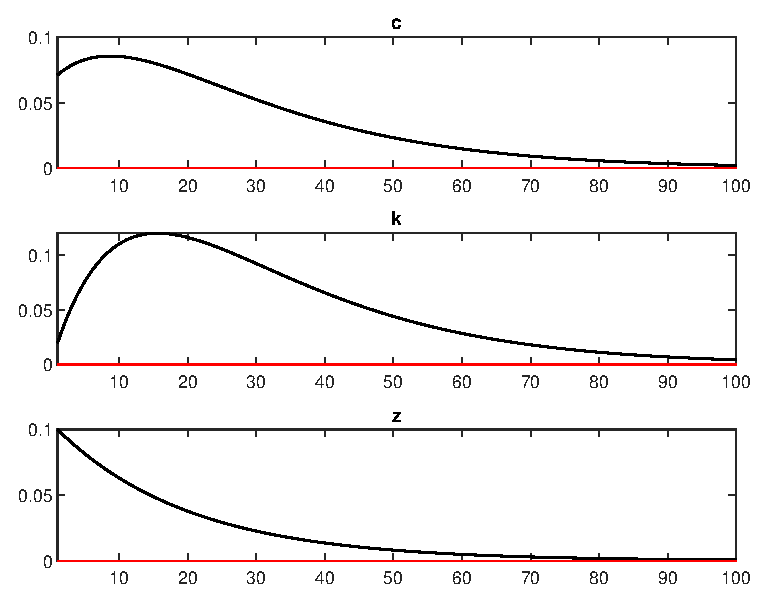
\includegraphics[width=0.7\linewidth]{../figs/stochastic_growth_dynare_IRF_e}
\end{figure}

\begin{itemize}
	\item \small IRF of $ c,k $ and $ z $ to a 1 st.dev. shock to $ \varepsilon $.
	
\end{itemize}

\end{frame}
%%%%%%%%%%%%%%%%%%%%%%%%%%%%%%%%%%%%%%%%%%%%%%

\begin{frame}[fragile]
\frametitle{Dynare output}
\framesubtitle{Impulse responses, cont'd}

\begin{itemize}
	\item By default, Dynare plots IRFs of all endogenous variables.
	\item What if you are interested only in a subset of them? 
	\begin{itemize}
		\item E.g. only consumption and capital, not technology
	\end{itemize}
	\item Change \texttt{stoch\_simul} command as follows:
	\begin{verbatim}
	stoch_simul(order=1,irf=100) c k;
	\end{verbatim}
\end{itemize}


\begin{figure}
	\centering
	\includegraphics[width=0.5\linewidth]{"../figs/stochastic_growth_dynare_IRF_e (2)"}
\end{figure}

	
\end{frame}
%%%%%%%%%%%%%%%%%%%%%%%%%%%%%%%%%%%%%%%%%%%%%%


\begin{frame}[fragile]
\frametitle{Dynare output}
\framesubtitle{Matlab workspace}
\begin{itemize}
	\item Where does Dynare store results?
\end{itemize}
\begin{figure}
	\centering
	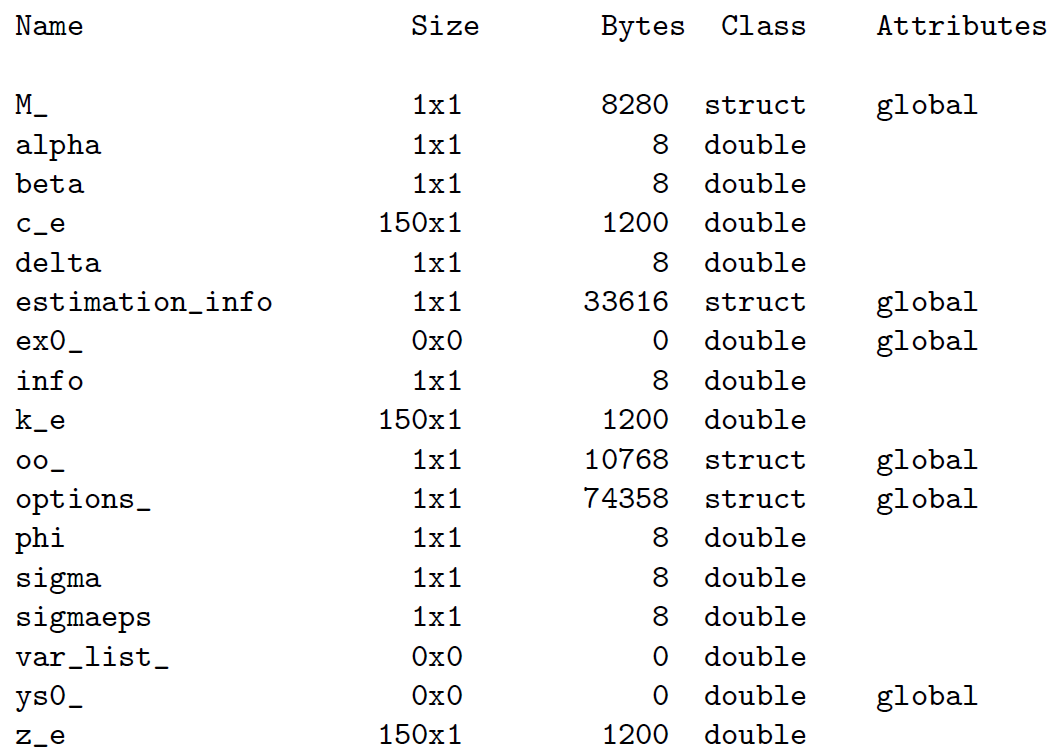
\includegraphics[width=0.7\linewidth]{../figs/matlabwork}
	%\caption{}
	%\label{fig:matlabwork}
\end{figure}

\end{frame}
%%%%%%%%%%%%%%%%%%%%%%%%%%%%%%%%%%%%%%%%%%%%%%%%%%%%%%%%

\begin{frame}[fragile]
\frametitle{Dynare output}
\framesubtitle{Matlab workspace}
\begin{itemize}
	\item \textcolor{blue}{Parameters} that we supplied:
	\begin{verbatim}
	alpha, beta, delta, rho, sigma, sigmaeps
	\end{verbatim}
	\item \textcolor{blue}{Impulse responses} of each endogenous variable to each shock:
	\begin{verbatim}
	c_e, k_e, z_e
	\end{verbatim}
	\item Specialized \textcolor{red}{Matlab structures} that store key results:
	\begin{verbatim}
	M_, options_, oo_, ...
	\end{verbatim}
	\item \small These structures are also saved in \texttt{stochastic\_growth\_dynare\_results.mat}
	created by running Dynare on \texttt{stochastic\_growth\_dynare.mod}.
\end{itemize}
\end{frame}
%%%%%%%%%%%%%%%%%%%%%%%%%%%%%%%%%%%%%%%%%%%%%%%%%%%%%%%%

\begin{frame}[fragile]
\frametitle{Dynare output}
\framesubtitle{Structures}
\begin{itemize}
	\item Structures created by Dynare
	\begin{itemize}
		\item \texttt{M\_}, information about the model
		\item \texttt{options\_}, options used during computation
		\item \texttt{oo\_}, results of the computation
	\end{itemize}
	\item Get structure entries by ``\texttt{structure\_.entry}'', for example
	\begin{verbatim}
	oo_.steady_state
	\end{verbatim}
	recovers the steady state values given on a previous slide.
	\item \textcolor{red}{Warning}: Structure entries can be relatively complicated objects!!
\end{itemize}
\end{frame}
%%%%%%%%%%%%%%%%%%%%%%%%%%%%%%%%%%%%%%%%%%%%%%%%%%%%%%%%

\begin{frame}[fragile]
\frametitle{Dynare output}
\framesubtitle{Structures}
\begin{itemize}
	\item For example, the entries of \texttt{oo\_} are
\end{itemize}
\begin{figure}
	\centering
	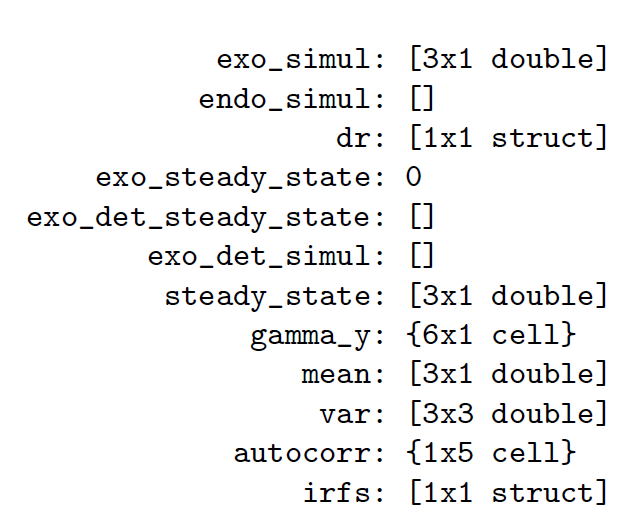
\includegraphics[width=0.7\linewidth]{../figs/oo_entries}
%	\caption{}
%	\label{fig:ooentries}
\end{figure}

\end{frame}
%%%%%%%%%%%%%%%%%%%%%%%%%%%%%%%%%%%%%%%%%%%%%%%%%%%%%%%%

\begin{frame}[fragile]
\frametitle{Dynare output}
\framesubtitle{Structures}
\begin{itemize}
	\item Structures can be nested into each other.
	\item Here, \texttt{oo\_.irfs} is another structure!
	\item If you type \texttt{oo\_.irfs} in the command window...
	\medskip 
	\begin{verbatim}
	 struct with fields:
	c_e: [1*100 double]
	k_e: [1*100 double]
	z_e: [1*100 double]
	\end{verbatim}
\end{itemize}
\end{frame}
%%%%%%%%%%%%%%%%%%%%%%%%%%%%%%%%%%%%%%%%%%%%%%%%%%%%%%%%

\begin{frame}[fragile]
\frametitle{Dynare output}
\framesubtitle{Decision rules structures}
\begin{itemize}
	\item Where does Dynare store the matrices of the state-space form solution?
\end{itemize}
\begin{verbatim}
POLICY AND TRANSITION FUNCTIONS
            c               k               z
Constant    0.186403        1.276779               0
k(-1)       0.382458        0.924091               0
z(-1)       0.676055        0.187070        0.950000
e           0.711637        0.196916        1.000000
\end{verbatim}
\end{frame}
%%%%%%%%%%%%%%%%%%%%%%%%%%%%%%%%%%%%%%%%%%%%%%%%%%%%%%%%

\begin{frame}[fragile]
\frametitle{Dynare output}
\framesubtitle{Decision rules structures}
\begin{itemize}
	\item Where does Dynare store the matrices of the state-space form solution?
	\item \texttt{oo\_.dr.ghx} is the $ 3\times2 $ matrix:
	\begin{verbatim}
	0.9241    0.1871
	0         0.9500
	0.3825    0.6761
	\end{verbatim}
	\item while \texttt{oo\_.dr.ghu} is the $ 3\times1 $ matrix
	\begin{verbatim}
	0.1969
	1.0000
	0.7116
	\end{verbatim}
\end{itemize}

\end{frame}
%%%%%%%%%%%%%%%%%%%%%%%%%%%%%%%%%%%%%%%%%%%%%%%%%%%%%%%%

\begin{frame}[fragile]
\frametitle{Dynare output}
\framesubtitle{Decision rules structures}
\begin{itemize}
	\item To simplify, let \texttt{oo\_.dr.ghx} be $ g_{x} $ and \texttt{oo\_.dr.ghu} be $ g_{u} $.
	\item From the above, can see that Dynare gives the state-space solution in the following format:
	\begin{equation*}
	\begin{bmatrix}
	k_{t} \\ 
	z_{t} \\ 
	c_{t}
	\end{bmatrix} =\underbrace{\begin{bmatrix}
		0.9241 & 0.1871  \\ 
		0 & 0.95  \\ 
		0.3825 & 0.6761   
		\end{bmatrix} }_{g_{x}}
	\begin{bmatrix}
	k_{t-1}\\ 
	z_{t-1}
	\end{bmatrix} + \underbrace{\begin{bmatrix}
		0.1969\\ 
		1\\ 
		0.7116
		\end{bmatrix}}_{g_{u}} \varepsilon_{t}  
	\end{equation*}
	\item Even if in the \texttt{*.mod} file we ordered the variables as ``c, k, z'', Dynare orders them as ``k, z, c''.
	\item For policy functions matrices $ g_{x} $ and $ g_{u} $ unfortunately Dynare does NOT follow the order of declaration chosen by the user, but the so-called DR-order.
\end{itemize}

\end{frame}
%%%%%%%%%%%%%%%%%%%%%%%%%%%%%%%%%%%%%%%%%%%%%%%%%%%%%%%%

\begin{frame}[fragile]
\frametitle{Dynare output}
\framesubtitle{Decision rules structures, cont'd}
\begin{itemize}
	\item \textcolor{blue}{Declaration order} chosen by the user: 
	\begin{itemize}
		\item In our example, the declaration order is ``c, k, z''.
	\end{itemize}
	\item \textcolor{red}{DR-order} (DR stands for decision rules): 
	\begin{itemize}
		\item Static variables
		\item State/backward looking variables
		\item Control/forward looking variables
	\end{itemize}
    \item Within each category, variables are arranged according to the declaration order.
    \begin{itemize}
    	\item In our example, the DR-order is ``k, z, c''. (There are no static variables).
    \end{itemize}
    \item More on this and other advanced Dynare topics in the next class.
\end{itemize}

\end{frame}
%%%%%%%%%%%%%%%%%%%%%%%%%%%%%%%%%%%%%%%%%%%%%%%%%%%%%%%%





\begin{frame}
\begin{center}
	{\Large Dynare: Advanced features}
\end{center}
\end{frame}

\begin{frame}[fragile]
\frametitle{Peculiarities of Dynare: timing convention}
%\framesubtitle{subtitle}
\begin{itemize}
	\item All variables known at time $ t $ must be dated $ t-1 $ (i.e. $ k_{t} $ is a choice variable, $ k_{t-1}$ is a state or predetermined variable).
	\item This is different from convention used in most of the macro literature.
	\item Can change this timing convention using the \texttt{predetermined\_variables} command.
	\item The following two examples are \underline{exactly} equivalent.
\end{itemize}
\end{frame}
%%%%%%%%%%%%%%%%%%%%%%%%%%%%%%%%%%%%%%%%%%%%%%%%%%%%%%%%

\begin{frame}[fragile]
\frametitle{Peculiarities of Dynare: timing convention, cont'd}
\small 
\begin{columns}[c]
	
	
	\column{.45\textwidth} % Left column and width
	
	Using \textcolor{blue}{default} Dynare timing convention:
	\begin{verbatim}
	var y, k, i;
	…
	model;
	y = k(-1)^alpha;
	k = i + (1-delta)*k(-1);
	…
	end;
	\end{verbatim}
	
	
	
	\column{.5\textwidth} % Right column and width
	
	
	Using the \textcolor{red}{alternative} timing convention:
	\begin{verbatim}
	var y, k, i;
	predetermined_variables k;
	…
	model;
	y = k^alpha;
	k(+1) = i + (1-delta)*k;
	…
	end;
	\end{verbatim}
	


\end{columns}

\end{frame}
%%%%%%%%%%%%%%%%%%%%%%%%%%%%%%%%%%%%%%%%%%%%%%%%%%%%%%%%

\begin{frame}[fragile]
\frametitle{Adding extra variables}
%\framesubtitle{subtitle}
\begin{itemize}
	\item Suppose you would like to include also output and interest rate in your analysis.
	\item Modify the \texttt{*.mod} file as follows.
	\item Change (1) by adding the extra variables
	\begin{verbatim}
	// (1) declare endogenous variables
    var  c, k, y, r, z;
	\end{verbatim}
	\item Change model equations in (4) by adding
	\begin{verbatim}
	// Output
	y = exp(z)*(exp(k(-1))^alpha);
	// Interest rate
	r = alpha*exp(z)*(exp(k(-1))^(alpha-1));
	\end{verbatim}
\end{itemize}
\end{frame}

\begin{frame}[fragile]
\frametitle{Adding extra variables, cont'd}
%\framesubtitle{subtitle}
\begin{itemize}
	\item Finally, you need to provide initial conditions in the steady-state block (5) also for the new variables:
	\begin{verbatim}
	initval;
	c = 0.75;
	k = 3;
	z = 1;
	e = 0;
	y = exp(3)^alpha;
	r = alpha*(exp(3)^(alpha-1));
	end;
	\end{verbatim}
\end{itemize}
\end{frame}
%%%%%%%%%%%%%%%%%%%%%%%%%%%%%%%%%%%%%%%%%%%%%%

\begin{frame}[fragile]
\frametitle{Linear model}
%\framesubtitle{subtitle}
\begin{itemize}
	\item Suppose you have already log-linearized your model equations.
	\item Or you prefer to work with linearized solution for any reason
	\begin{itemize}
		\item Common for the three-equations New-keynesian model.
	\end{itemize}
    \item Then you should add option ``linear'' to your model block declaration:
    \begin{verbatim}
    model(linear);                                   
    
    end;
    \end{verbatim}
    \item The option ``linear'' tells Dynare your model is already linear and thus speeds up some computations. 
    \item However, when your model is already linear, not putting ``linear'' does of course not influence the results. 
    \begin{itemize}
    	\item A linear approximation of a linear equation is simply the equation itself!
    \end{itemize} 
\end{itemize}
\end{frame}

\begin{frame}[fragile]
\frametitle{Loops over parameters}
%\framesubtitle{subtitle}
\begin{itemize}
	\item This trick allows you to run the same Dynare program for
	different parameter values.
	\item Suppose your Dynare program has the command
	\begin{verbatim}
	rho=0.8;
	\end{verbatim}
	\item You would like to run the program twice; once for $ \rho=0.8 $, and
	once for $ \rho=0.9 $.
	\item Of course you could write two separate \texttt{*.mod} files, one for each parameter value.
	\item But there is a better solution...
\end{itemize}
\end{frame}
%%%%%%%%%%%%%%%%%%%%%%%%%%%%%%%%%%%%%%%%%%%%%%%%%%%%%%%%

\begin{frame}[fragile]
\frametitle{Loops over parameters, cont'd}
%\framesubtitle{subtitle}
\begin{enumerate}
	\item In your Matlab program, loop over the different values of rho.
	Save the value of rho and the associated name to the file ``parameterfile'':
	\begin{verbatim}
	save parameterfile rho
	\end{verbatim}
	and \textit{then} run Dynare.
	\item In your Dynare program file, replace the command \texttt{rho=0.8} with:
	\begin{verbatim}
	load parameterfile
	set_param_value('rho',rho);
	\end{verbatim}
	
\end{enumerate}

\begin{itemize}
	\item Remarks:
	\begin{itemize}
		\item The name of the file is arbitrary.
		\item In \texttt{set\_param\_value('.',.)}, the first argument is the name in your *.mod file and the second is the numerical value.
	\end{itemize}
\end{itemize}

\end{frame}

\end{document}
